\chapter{集成运算放大电路}
除了放大模拟信号,也需要对信号进行各种运算。而基本放大电路难以实现这些运算,因此引入多级放大电路,并制成了集成运算放大器。本章将会先简单介绍多级放大电路,然后介绍集成运放对每一级相应的电路,最后讲解对集成运放的特性及运算电路。

\section{多级放大电路}
放大电路中每一个基本放大电路称为一级,而将它们连接起来就称为\textbf{级间耦合}\index{J!级间耦合}。

\subsection{耦合方式}

\subsubsection{一、直接耦合}
最简单的连接方式就是将前一级的输出端直接连接到后一级的输入端,这种称为\textbf{直接耦合}\index{Z!直接耦合}。由于各级之间是直接连接起来的,静态工作点会相互影响,且存在零漂现象。

\subsubsection{二、阻容耦合}
为了避免静态工作点相互影响,会使用电容连接电路的两级,称为\textbf{阻容耦合}\index{Z!阻容耦合}。由于存在电容,会导致低频信号难以通过,且难以集成到一片硅片上。

\subsection{多级放大电路的动态分析}
多级放大电路的电压放大倍数就是各级电压放大倍数的乘积,其中值得注意的是,每一级的放大倍数应当是以后级的输入电阻作为负载时的放大倍数。多级放大电路的输入电阻就是第一级的输入电阻,而输出电阻就是最后一级的输出电阻。

在计算的过程中,需要注意必须将第二级的输入电阻作为第一级的负载,计算在第一级的增益之内。

\section{电流源电路}
在集成电路中,制作一个三极管比制作一个电阻所占用的面积更小,因此往往会选择三极管构成直流电流源,常用于在电路中提供静态偏置,或者充当大电阻。

\subsection{镜像电流源}\index{J!镜像电流源}
图\ref{BJT镜像电流源电路}为BJT镜像电流源电路。对静态工作点进行分析,可以得到\textbf{基准电流}\index{J!基准电流}
\begin{equation}
    I_{\mathrm{REF}}=\frac{V_{\mathrm{CC}}-V_{\mathrm{BE}}-(-V_{\mathrm{EE}})}{R}
\end{equation}

由对称性和节点电流法,可以得到
\begin{equation}
    I_\mathrm{O}=I_{\mathrm{C2}}=\frac{I_{\mathrm{REF}}}{1+2/\beta}
\end{equation}

可见,电流大小与负载无关。而其输出电阻为
\begin{equation}
    r_{\mathrm{o}}=r_{\mathrm{ce2}}=\frac{1}{\lambda I_{\mathrm{C2}}}
\end{equation}

因此其输出电阻很大,可以在电路中取代大电阻。

实际上,在$V_{\mathrm{CC}}$一定的情况下,如果要求$I_{\mathrm{C2}}$很大,则需要$I_{\mathrm{REF}}$很大,导致电阻上的功耗增加,这应当避免。如果要求$I_{\mathrm{C2}}$很小,则需要$I_{\mathrm{REF}}$很小,此时需要电阻$R$很大,也应当避免。因此派生了其他类型的电流源。

\begin{figure}[htb]
    \centering
    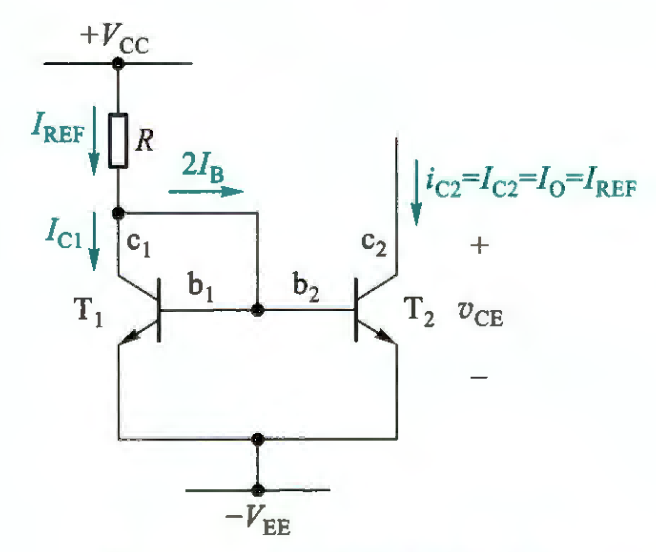
\includegraphics[width=0.5\linewidth]{pic/BJT镜像电流源电路.png}
    \caption{BJT镜像电流源电路\cite{康华光}\label{BJT镜像电流源电路}}
\end{figure}

\subsection{比例电流源}
\textit{(本节的内容仅做了解)}

比例电流源如图\ref{比例电流源}所示。由电路可知
\begin{equation}
    V_{\mathrm{BE0}}+I_{\mathrm{E0}}R_{\mathrm{e0}}=V_{\mathrm{BE1}}+I_{\mathrm{E1}}R_{\mathrm{e1}}
\end{equation}

而BJT管的发射结电压和发射结电流之间的关系近似为(这里不再使用恒压降模型)
\begin{equation}
    V_{\mathrm{BE}}=V_{\mathrm{T}}\ln \frac{I_{\mathrm{E}}}{I_{\mathrm{S}}}
\end{equation}

其中$V_{\mathrm{T}}$为电压当量,因此
\begin{equation}
    I_{\mathrm{E1}}R_{\mathrm{e1}}-I_{\mathrm{E0}}R_{\mathrm{e0}}\approx V_{\mathrm{T}}\ln \frac{I_{\mathrm{E0}}}{I_{\mathrm{E1}}}
\end{equation}

由于$I_{\mathrm{C0}}\approx I_{\mathrm{E0}}\approx I_{\mathrm{R}}$,$I_{\mathrm{C1}}\approx I_{\mathrm{E1}}$,则
\begin{equation}
    I_{\mathrm{C1}}\approx \frac{R_{\mathrm{e0}}}{R_{\mathrm{e1}}}I_\mathrm{R}+\frac{V_{\mathrm{T}}}{R_{\mathrm{e1}}}\ln \frac{I_{\mathrm{R}}}{I_{\mathrm{C1}}}
\end{equation}

在一定范围内,对数项可以忽略,因此$I_{\mathrm{C1}}$与$I_{\mathrm{R}}$成正比。只要改变$R_{\mathrm{e0}}$和$R_{\mathrm{e1}}$的关系,就可以改变$I_{\mathrm{C1}}$与$I_{\mathrm{R}}$的比例关系。

\begin{figure}[htb]
    \centering
    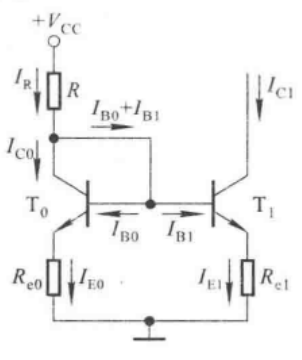
\includegraphics[width=0.3\linewidth]{pic/比例电流源.png}
    \caption{比例电流源\cite{华成英}\label{比例电流源}}
\end{figure}

\subsection{微电流源}
在比例电流源的基础上取$R_{\mathrm{e0}}=0$,就构成了微电流源。

\section{差分放大电路}
由于阻容耦合中会出现大量的电容,不便于集成,因此在集成电路中仍会采用直接耦合的方式,但直接耦合会产生零点漂移的现象。\textbf{零点漂移}\index{L!零点漂移},顾名思义,就是输入电压被置零但输出电压随时间变化的现象。

后来,人们想出了一个对称的构造——差分放大电路,并将其作为集成放大电路的输入级,有效地抑制了零点漂移的现象。本节仅讨论BJT构成的差分放大电路。

\subsection{差模信号与共模信号及相关参数}
差分放大电路的整体结构非常对称,这样就消除了各种各样的干扰和噪声。各种干扰的信号由于是对两边同步输入就变成了共模信号,在输出时一作差就被消除了,而需要的信号变成了差模信号。为了更好地讨论差分放大电路的性能,引入如下概念。

\subsubsection{一、信号}
在电路中,信号有两个输入端:同相输入端$v_{\mathrm{P}}$和反相输入端$v_{\mathrm{N}}$,其中下标字母P和N分别表示positive和negative。

另一种分类方式为差模信号和共模信号,其定义如下:

1.\textbf{差模信号}\index{X!信号!差模信号}:定义为两输入端信号的差值,即$v_{\mathrm{id}}=v_{\mathrm{P}}-v_{\mathrm{N}}$,其中下标字母d的含义为differential。

2.\textbf{共模信号}\index{X!信号!共模信号}:定义为两输入端信号的算数平均值,即$v_{\mathrm{ic}}=(v_{\mathrm{P}}+v_{\mathrm{N}})/2$,其中下标字母c的含义为common。

\subsubsection{二、增益}
1.\textbf{差模电压增益}\index{F!放大倍数!差模电压增益}:即仅考虑差模信号输入时的电压增益$A_{\mathrm{vd}}=v_{\mathrm{od}}/v_{\mathrm{id}}$。

2.\textbf{共模电压增益}\index{F!放大倍数!共模电压增益}:即仅考虑共模信号输入时的电压增益$A_{\mathrm{vc}}=v_{\mathrm{oc}}/v_{\mathrm{ic}}$。

则总输出为
\begin{equation*}
    v_\mathrm{o}=v_\mathrm{od}+v_\mathrm{oc}=A_\mathrm{vd}v_\mathrm{id}+A_\mathrm{vc}v_\mathrm{ic}
\end{equation*}

\subsubsection{三、共模抑制比}
为了反映电路放大差模信号和抑制共模信号的综合能力,引入\textbf{共模抑制比}\index{G!共模抑制比}$K_{\mathrm{CMR}}=|A_{\mathrm{vd}}/A_{\mathrm{vc}}|$,下标CMR表示common mode rejection。

另外需要注意的是,\textbf{这里讨论的输入信号都是交流小信号},而非直流信号。

\subsection{差分放大电路的分析}
差分放大电路特殊的地方在于它的两个输入端都是有效输入端,而非一个输入端接地,这也导致其分为双端输入和单端输入。实际上,差分放大电路的输入和输出都可以有单端和双端两种,因此一共有四种组合。

通常,两个BJT的射极会接在同一个恒流源(如镜像电流源),导致电路中看起来有很多管子。但其实只要按照功能将一个个模块分解开就知道并不复杂。

\subsubsection{一、静态分析}
在静态分析的时候直接将两个基极接地即可。由于发射极接了恒流源,静态分析并不困难,此处从略。

\subsubsection{二、动态分析}
在动态分析的时候,通常需要将共模信号和差模信号分开讨论。

\begin{figure}[htb]
    \centering
        \subcaptionbox{输入差模信号时\cite{康华光}\label{输入差模信号时的交流通路}}
        {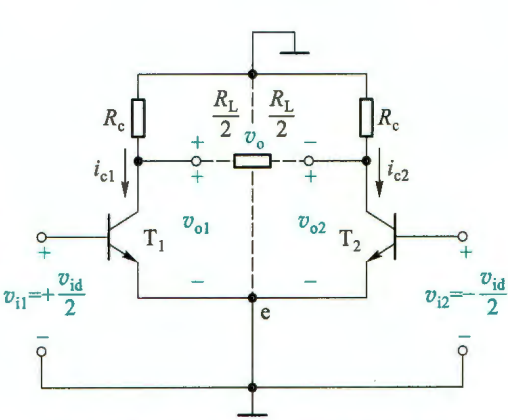
\includegraphics[width=0.45\textwidth]{pic/输入差模信号时的交流通路.png}}\qquad
        \subcaptionbox{输入共模信号时\cite{康华光}\label{输入共模信号时的交流通路}}
        {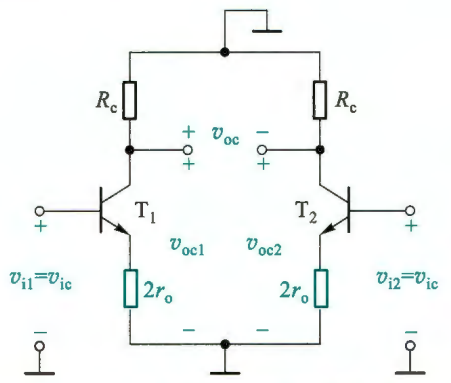
\includegraphics[width=0.45\textwidth]{pic/输入共模信号时的交流通路.png}}
        \caption{输入不同信号时的交流通路\label{输入不同信号时的交流通路}}
\end{figure}

\textbf{1.差模信号的增益}

输入差模信号时的交流通路如图\ref{输入差模信号时的交流通路}所示。在分析差模信号时,考虑到电路理想对称,对称轴上电压为0,相当于全部接地。

a.双端输入、单端输出时

不接负载时,在$v_{\mathrm{o1}}$端输出的电压增益为
\begin{equation}
    A_{v\mathrm{d1}}=-\frac{\beta R_\mathrm{c}}{2r_\mathrm{be}}
\end{equation}

接上负载后$R_\mathrm{L}$,在$R_\mathrm{c}$上并上负载电阻$R_\mathrm{L}$即可。

对于差模电压增益,从两个口输出的区别在于其相位不同,相差一个负号。

b.双端输入、双端输出时

在不接负载的情况下,双端输出的差模电压增益是单端输出的2倍,与单管的电路增益相同,相当于用双倍的元件换取了抑制零漂的能力。虽然它的差模增益更高,但是没有对地输出使得它不如单端输出稳定。

如果接上负载,利用对称性,等效于单边并上了一个$R_\mathrm{L}/2$的电阻,电压增益为
\begin{equation}
    A_{v\mathrm{d}}=-\frac{\beta R_\mathrm{c} \parallel (R_\mathrm{L}/2)}{r_\mathrm{be}}
\end{equation}

c.单端输入时

差模信号的单端输入必然伴随着共模信号的输入。单端输入可以等效为双端输入,因此单端输入和双端输入的差模增益指标相同。

\textbf{2.共模信号的增益}

输入共模信号时,由于此时射极电压不再为0,电流源的内阻不可忽略。如果保持射极电压不变,可以将$r_\mathrm{o}$分别等效到两端支路上,如图\ref{输入共模信号时的交流通路}所示。

由于共模输入两端信号完全相同,输入时没有单端输入和双端输入之分。

a.双端输出时

由于两边完全对称,共模电压增益为0,共模抑制比$K_{\mathrm{CMR}}=\infty$。

b.单端输出时

共模电压增益类似基本共射放大电路的电压增益,只是将$R_\mathrm{e}$替换为了$2r_\mathrm{o}$:
\begin{equation}
    A_{v\mathrm{c}}=-\frac{\beta R_\mathrm{c}}{r_\mathrm{be}+(1+\beta)2r_\mathrm{o}}\approx -\frac{R_\mathrm{c}}{2r_\mathrm{o}}
\end{equation}
此时共模抑制比$K_{\mathrm{CMR}}$有限。

\textbf{3.输入电阻和输出电阻}

差模输入电阻
\begin{equation}
    R_\mathrm{id}=2r_\mathrm{be}
\end{equation}

共模输入电阻
\begin{equation}
    R_\mathrm{ic}=\frac{1}{2}[r_\mathrm{be}+(1+\beta)(2r_\mathrm{o})]
\end{equation}

单端输出时的输出电阻
\begin{equation}
    R_\mathrm{o}=R_\mathrm{c}
\end{equation}

双端输出时的输出电阻是单端输出的两倍
\begin{equation}
    R_\mathrm{o}=2R_\mathrm{c}
\end{equation}

\textbf{实际上,对于这些结论,只要按照之前的动态分析方法,将BJT替换为相应的小信号模型就能直接算出来。}图\ref{差分放大电路四种接法的比较}中汇总了几种电路相关结论,注意原来的直流源被替换成了射极电阻$R_\mathrm{e}$。

\begin{figure}[htb]
    \centering
    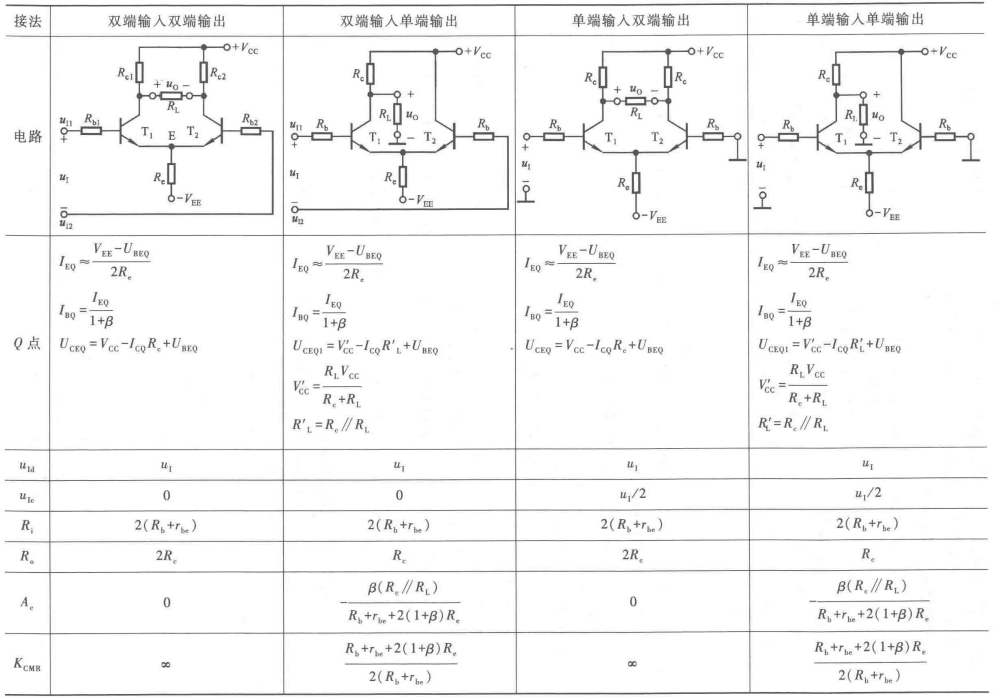
\includegraphics[width=0.95\linewidth]{pic/差分放大电路四种接法的比较.png}
    \caption{差分放大电路四种接法的比较(图片来源:康华光指导92页)\label{差分放大电路四种接法的比较}}
\end{figure}

\section{直接耦合互补输出级}
\textit{(本节的内容仅做了解)}
上一节讲解的差分放大器,往往用于多级放大电路的输入级,将零漂扼杀于摇篮之中。而在输出级,一般要求输出电阻低,且最大不失真输出电压尽可能大,因此产生了直接耦合互补输出级。如图\ref{互补射极输出电路}所示。互补输出级也常作为功率放大电路。

\begin{figure}[htb]
    \centering
    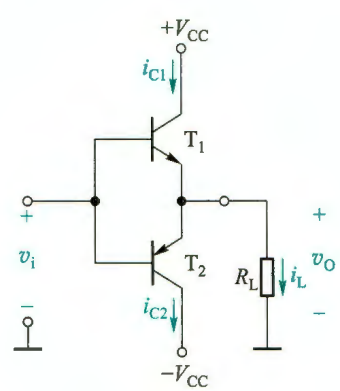
\includegraphics[width=0.25\linewidth]{pic/互补射极输出电路.png}
    \caption{互补射极输出电路\cite{康华光}\label{互补射极输出电路}}
\end{figure}

\section{集成运算放大器}
将上述各单元电路组合起来,就可以构成一个\textbf{集成电路运算放大器},简称为\textbf{集成运放}。

集成运放通常由至少三级放大电路构成。比较常见的构成是,输入级为CMOS差分放大电路作为输入,中间级为共射放大电路,输出为功率放大电路作为输出。其中,第一级将电路的两个输入端口作差抑制共模信号,第二级让信号放大,第三级再次放大并且提供比较好的输出匹配。这样就得到了一个输入电阻高、输出电阻低、增益系数大的放大电路模块。

集成运放由于其近似理想的特性备受关注,并且多用于各种模拟信号的运算。由于其内部结构复杂,本节将集成运放作为一个黑匣子,讨论集成运放的外部特性,并简单介绍集成运放的应用电路。

\subsection{运算放大器的特性}
运算放大电路的简化模型如图\ref{运算放大器的电路简化模型}所示,其中供电电源通常会被省略,只会在必要时画出。

\begin{figure}[htb]
    \centering
    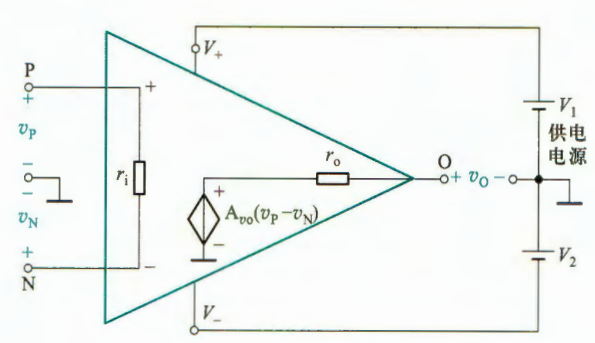
\includegraphics[width=0.55\linewidth]{pic/运算放大器的电路简化模型.png}
    \caption{运算放大器的电路简化模型\cite{康华光}\label{运算放大器的电路简化模型}}
\end{figure}

由于输入级为差分放大电路,输出电压与输入级电压之差成正比,即$v_{\mathrm{O}}=A_{v\mathrm{o}}(v_{\mathrm{P}}-v_{\mathrm{N}})$。其中$A_{v\mathrm{o}}$为\textbf{开环电压增益}\index{K!开环电压增益},而P表示\textbf{同相输入端}\index{S!输入端!同相输入端},N表示\textbf{反相输入端}\index{S!输入端!反相输入端}。此外,在图\ref{运算放大器的电路简化模型}中还可以看到输入电阻$r_\mathrm{i}$和输出电阻$r_\mathrm{o}$。

但实际上,由于工作电源的限制,\textbf{线性工作区}\index{X!线性工作区}很小。当$A_{v\mathrm{o}}(v_{\mathrm{P}}-v_{\mathrm{N}})$过大时,会进入\textbf{饱和区}\index{B!(集成运放)饱和区}。

对于集成运放,同样有差模信号、共模信号、共模抑制比等等定义,可以直接类比差分放大电路对应的概念。由于输出电压只与差模信号有关,因此共模电压增益为0,共模抑制比为无穷。

\subsection{理想运算放大器}
为了简化电路分析,人们将集成运放的各项指标理想化,就能得到理想的运放模型。

对于理想的运算放大器,最重要的两个性质为:

1.开环电压增益$A_{v\mathrm{o}}=\infty$,但输出电压为有限值,因此$v_{\mathrm{P}}=v_{\mathrm{N}}$,称为“\textbf{虚短}”。

2.输入电阻$r_{\mathrm{i}}=\infty$,此时$i_{\mathrm{P}}=i_{\mathrm{N}}=0$,称为“\textbf{虚断}”。

此外,还会认为其输出电阻$r_{\mathrm{o}}=0$。

\subsection{运算放大器的应用电路}
由于集成运放的开环增益极高,线性区$(v_{\mathrm{P}}-v_{\mathrm{N}})$非常小,难以保证其工作在线性区,因此需要引入负反馈来减小$(v_{\mathrm{P}}-v_{\mathrm{N}})$的值,也就是让其工作在闭环状态。

本节仅简单讨论最基本的运放应用电路之一——同相放大电路,如图\ref{同相放大电路}所示。

\begin{figure}[htb]
    \centering
    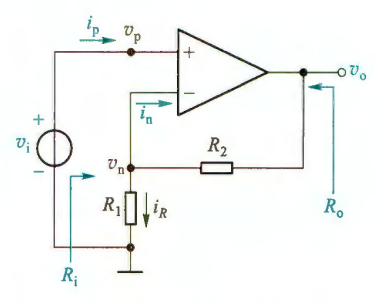
\includegraphics[width=0.45\linewidth]{pic/同相放大电路.png}
    \caption{同相放大电路\cite{康华光}\label{同相放大电路}}
\end{figure}

在运放的反相端运用KCL,得到
\begin{equation}
    \frac{v_\mathrm{o}-v_\mathrm{n}}{R_2}=\frac{v_\mathrm{n}}{R_1}+i_\mathrm{n}
\end{equation}

再利用$v_{\mathrm{p}}=v_{\mathrm{n}}=v_{\mathrm{i}}$和$i_{\mathrm{p}}=i_{\mathrm{n}}=0$,就得到
\begin{equation}
    A_v=1+\frac{R_2}{R_1}
\end{equation}

除了同相放大电路外,还有以下基本应用:
\begin{itemize}
    \item 反相放大电路;
    \item 电压跟随器(缓冲器、隔离器);
    \item 求和电路、求差电路;
    \item 积分电路、微分电路;
\end{itemize}

此外,还有更复杂的对数电路、指数电路、乘法电路、除法电路……